\subsection{Muon System (8 p.)}
\subsubsection{Muon Tracking (Herve; 5p.)}
\subsubsection{Muon Identifier (Pascal; 3p.)}

The Muon Identifier (MID) is the present designation of the Muon Trigger system~\cite{Aamodt:2008zz} which was operational in ALICE during LHC run~1 and run~2. 

The detector is composed of 72 single gap Resistive Plate Chamber (RPC) detectors, organized in two stations of two planes each, located at 16~m and 17~m from 
the interaction point. The planes in the same station are 17~cm apart. The total detection area is about 150~m$^{\rm 2}$. An overview picture of one half-plane of the MID, in open position, taken during the FEERIC card 
installation (see next section) in 2019, is shown in Fig.~\ref{midhalfplaneopen}.

The RPC signals are collected by means of a total of 20992 readout strips, each of them equipped with Front-End (FE) electronics. The output signals from the FE electronics, in LVDS electrical standard of 25~ns width, 
are propagated via multi-wire copper cables to the readout electronics (also in charge of the muon trigger decision during run~1 and run~2). 

\begin{figure}
\centering 
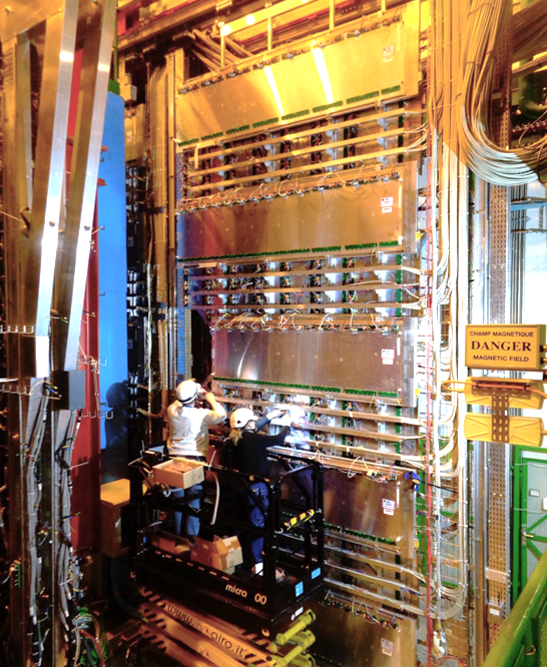
\includegraphics[width=.4\textwidth]{mid/midhalfplaneopen}
\caption{Overview of one MID half-plane in open position}
\label{midhalfplaneopen}
\end{figure}

The FE electronics cards, located on the RPC detectors, have been replaced during the LS2. The main motivation is to reduce the ageing of the RPCs during future data taking periods. 
The FE ASIC of the past FE electronics, called ADULT~\cite{mid:ADULT}, has been upgraded to a new one, called FEERIC~\cite{mid:FEERICref1,mid:FEERICref2}.
Unlike ADULT, FEERIC performs amplification of the RPC analog signals. Thanks to this upgrade, the ALICE RPCs will be operated in avalanche 
mode after the LS2 with a significant reduction of the charge produced in the gas gap as compared to past conditions, hence limiting ageing effects.

The readout electronics (more than 250 complex electronics cards) have been also completely replaced for sustaining the large data flow going with the future high collision rate. 
The new system is designed for continuous readout so there is no more need for hardwired muon trigger signals, the event selection being done at the online processing level. 

All RPC detectors were still operational at the end of run~2. However few of them were drawing a relatively large current after having accumulated up to 20~mC/cm$^{\rm 2}$.
It was therefore decided to replace those RPCs by completely new produced ones. For the longer term, a crucial R\&D on new environment-friendly 
gas mixtures~\cite{mid:RPCgasmix} for RPCs, based on tetrafluoropropene which is characterized by a very low Global Warning Potential (GWP), has been launched.


\paragraph{FEERIC electronics\\}
 
The FEERIC 8-channel ASIC is designed in the AMS 0.35~$\mu{\rm m}$ CMOS technology. It is mostly composed (see Fig.~\ref{midFEERIC}, top scheme) of a transimpedance amplifier, a zero-crossing discriminator and a one-shot 
which prevents retriggering during 100~ns. The operating threshold is typically 70~mV corresponding roughly to 130~pC at readout strip level. Details of the performance of the FEERIC electronics 
is given in~\cite{mid:FEERIC-PRR}. Figure~\ref{midFEERIC}, bottom, shows a picture of a FEERIC card. 2720 cards (spare included) have been produced in the second half of 2017.
The installation of the FEERIC cards on the RPCs in ALICE cavern has been completed in July 2019. 

In parallel, a new wireless threshold distribution for the FEERIC cards has been developed. 
A total of two masters (one per side of the cavern) and 24 nodes close from the RPCs (see Fig.~\ref{midTHRdistri}, picture on the right), installed in ALICE cavern in 2019, allows to remotely control the threshold of each of the 2384 installed 
FEERIC cards. The masters are controlled via ethernet and communicate via the high level ZIGBEE wireless protocol with the nodes which are themselves I2C chained to the FEERIC cards on the RPCs (see Fig.~\ref{midTHRdistri}, 
scheme on the left). Master and node share the same hardware and firmware. Card acts as master or node depending on the configuration stored in EEPROM which also keep memory of the last requested threshold values, restored
at power on.  

During run-2, one of the 72 ALICE RPCs was equipped with FEERIC electronics and the wireless distribution, showing satisfactory performance and stability. The charge released in the gas (25-30~pC per hit) is four times less 
than the one of RPCs with ADULT.

\begin{figure}
\centering 
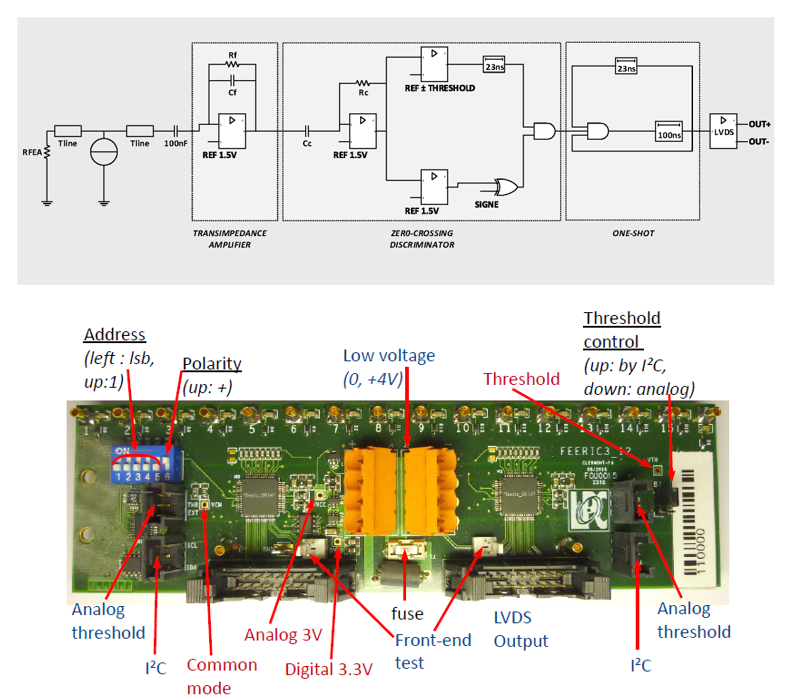
\includegraphics[width=.5\textwidth]{mid/midFEERIC}
\caption{FEERIC ASIC architecture (top) and FEERIC card picture (bottom)}
\label{midFEERIC}
\end{figure}

\begin{figure}
\centering 
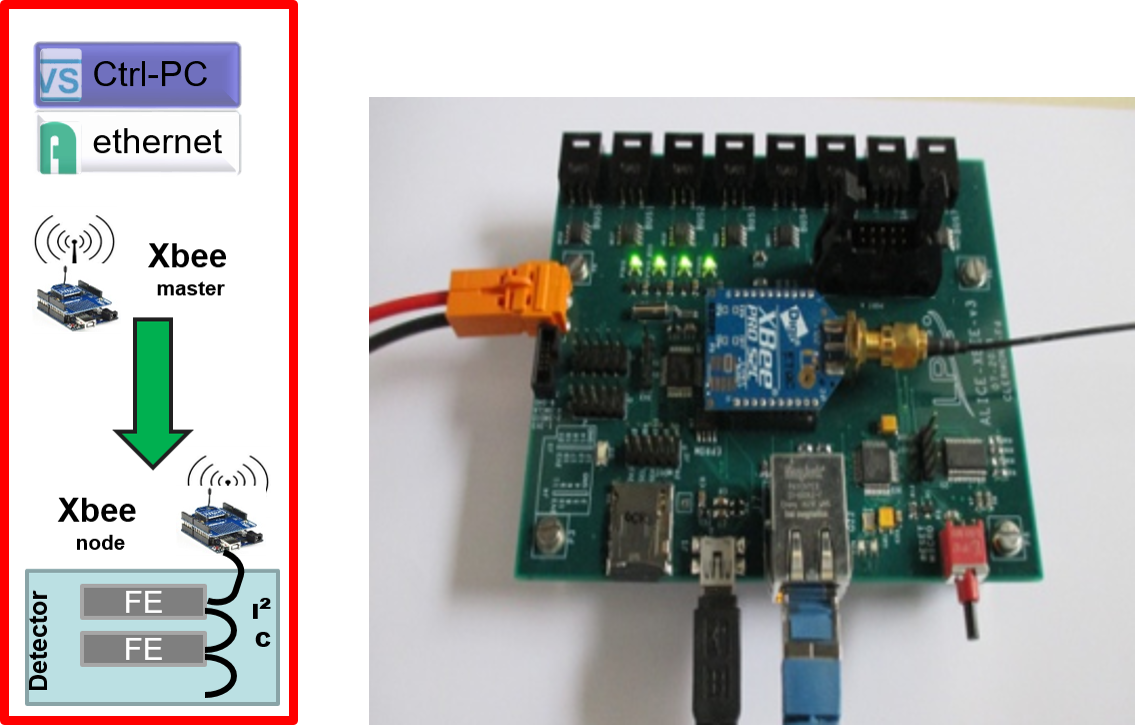
\includegraphics[width=.5\textwidth]{mid/midTHRdistri}
\caption{Wireless threshold distribution scheme (left) and master or node electronics card (right)}
\label{midTHRdistri}
\end{figure}




\paragraph{Readout electronics\\}

The LVDS (binary) signals from the FE electronics, so called strip-patterns of length 16 bits, are received by the Local cards. 
Each Local receives strip-patterns from the four detector planes, each of them from the two orthogonal coordinates (from horizontal and vertical readout strips on both sides 
of the same RPC). The whole project consists in 234 Local cards, housed in 16 VME-9U crates used as mechanical support and for power supply. 
The Regional card in the crate communicates with a maximum of 16 Local cards via the e-links of the J2 bus. Each Regional card is interfaced to a Common Readout Unit (CRU) by means of two GBT links at 3,2~Gbit/s. 

The project has a total of two CRUs only, housed in one single First Level Processor (FLP) tower PC. The MID readout architecture is shown in the left panel of Fig.~\ref{midRO} while a picture of the three types of readout cards 
is shown on the right. Simulations of the expected bandwidth for Pb--Pb collisions at 50~kHz, based on run~2 real data, indicate that 
this design includes a safety factor of more than one order of magnitude. 

Data corresponding to so-called self-triggered physics events~\cite{mid:ROweb,mid:DataNote} are transmitted from the Local and Regional to the CRU. There is potentially a new event stored 
in the Local and Regional FIFOs each 25~ns. Information is stored in these FIFOs only in case of a non-empty event which, in standard configuration,
corresponds to at least two coordinates in the same detector plane with non-zero bit-patterns. 
It is important to note that it takes five clock cycles (at 40~MHz) per self-triggered event for the transfer of the Regional FIFO and 9-21 clock cycles for the transfer of the Local FIFO, depending on the
number of non-empty planes in this last case. As a first consequence, the data from Local and Regional corresponding to the same bunch crossing (BC) arrive asynchronously in the CRU. As a second consequence, the
Local and Regional FIFOs would go to saturation in case of filling at the full clock frequency, corresponding for example to a very high level of noise at the FE level: a busy bit would be set in such case.

The CRU user logic (UL), first stage of data processing in the CRU, is essentially performing zero-suppression and raw data header construction using the central trigger (CTP) orbit information. 
The UL output is transmitted by words of 256 bits to the FLP. At this level, the data coming from the different GBT links are assembled in C++ structures and synchronized to provide the information 
corresponding to a given interaction. The readout electronics always operates in continuous readout mode. However the system can also handle triggered mode, selecting those events in coincidence with a trigger from the CTP, either 
in the CRU or the FLP.

The Local and Regional respond (see~\cite{mid:ROweb}) also to all types of central triggers issued by the CTP and received via the GBT down-link. 




\begin{figure}
\centering 
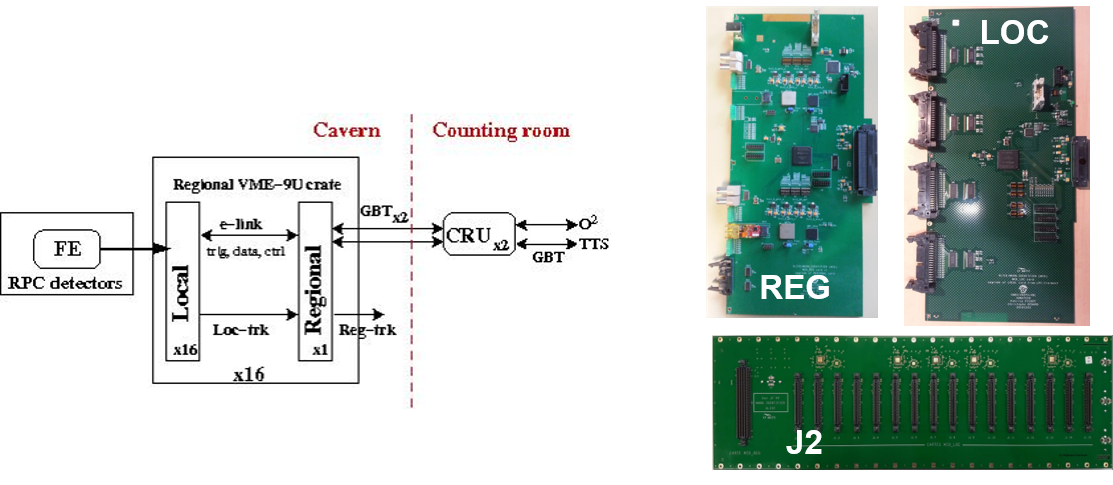
\includegraphics[width=1.\textwidth]{mid/midRO}
\caption{MID readout architecture (left) and readout cards (right picture) with Local (top right), Regional (top left) and J2 bus (bottom ) between Local and Regional}
\label{midRO}
\end{figure}





